\chapter{Inheritance}

In this chapter I present classes to represent playing cards,
decks of cards, and poker hands.  If you don't play poker, you can
read about it at \url{http://en.wikipedia.org/wiki/Poker}, but you don't have
to; I'll tell you what you need to know for the exercises.
Code examples from this chapter are available from
\url{http://thinkpython.com/code/Card.py}.
\index{playing card, Anglo-American}
\index{card, playing}
\index{poker}

If you are not familiar with Anglo-American playing cards,
you can read about them at \url{http://en.wikipedia.org/wiki/Playing_cards}.


\section{Card objects}

There are fifty-two cards in a deck, each of which belongs to one of
four suits and one of thirteen ranks.  The suits are Spades, Hearts,
Diamonds, and Clubs (in descending order in bridge).  The ranks are
Ace, 2, 3, 4, 5, 6, 7, 8, 9, 10, Jack, Queen, and King.  Depending on
the game that you are playing, an Ace may be higher than King
or lower than 2.
\index{rank}
\index{suit}

If we want to define a new object to represent a playing card, it is
obvious what the attributes should be: {\tt rank} and
{\tt suit}.  It is not as obvious what type the attributes
should be.  One possibility is to use strings containing words like
\verb"'Spade'" for suits and \verb"'Queen'" for ranks.  One problem with
this implementation is that it would not be easy to compare cards to
see which had a higher rank or suit.
\index{encode}
\index{encrypt}
\index{map to}
\index{representation}

An alternative is to use integers to {\bf encode} the ranks and suits.
In this context, ``encode'' means that we are going to define a mapping
between numbers and suits, or between numbers and ranks.  This
kind of encoding is not meant to be a secret (that
would be ``encryption'').

\newcommand{\mymapsto}{$\mapsto$}

For example, this table shows the suits and the corresponding integer
codes:

\begin{tabular}{l c l}
Spades & \mymapsto & 3 \\
Hearts & \mymapsto & 2 \\
Diamonds & \mymapsto & 1 \\
Clubs & \mymapsto & 0
\end{tabular}

This code makes it easy to compare cards; because higher suits map to
higher numbers, we can compare suits by comparing their codes.

The mapping for ranks is fairly obvious; each of the numerical ranks
maps to the corresponding integer, and for face cards:

\begin{tabular}{l c l}
Jack & \mymapsto & 11 \\
Queen & \mymapsto & 12 \\
King & \mymapsto & 13 \\
\end{tabular}

I am using the \mymapsto~symbol to make it clear that these mappings
are not part of the Python program.  They are part of the program
design, but they don't appear explicitly in the code.
\index{Card class}
\index{class!Card}

The class definition for {\tt Card} looks like this:

\begin{verbatim}
class Card(object):
    """Represents a standard playing card."""

    def __init__(self, suit=0, rank=2):
        self.suit = suit
        self.rank = rank
\end{verbatim}
%
As usual, the init method takes an optional
parameter for each attribute.  The default card is
the 2 of Clubs.
\index{init method}
\index{method!init}

To create a Card, you call {\tt Card} with the
suit and rank of the card you want.

\begin{verbatim}
queen_of_diamonds = Card(1, 12)
\end{verbatim}
%


\section{Class attributes}
\label{class.attribute}
\index{class attribute}
\index{attribute!class}

In order to print Card objects in a way that people can easily
read, we need a mapping from the integer codes to the corresponding
ranks and suits.  A natural way to
do that is with lists of strings.  We assign these lists to {\bf class
attributes}:

\begin{verbatim}
# inside class Card:

    suit_names = ['Clubs', 'Diamonds', 'Hearts', 'Spades']
    rank_names = [None, 'Ace', '2', '3', '4', '5', '6', '7', 
              '8', '9', '10', 'Jack', 'Queen', 'King']

    def __str__(self):
        return '%s of %s' % (Card.rank_names[self.rank],
                             Card.suit_names[self.suit])
\end{verbatim}
%
Variables like \verb"suit_names" and \verb"rank_names", which are
defined inside a class but outside of any method, are called
class attributes because they are associated with the class object 
{\tt Card}.
\index{instance attribute}
\index{attribute!instance}

This term distinguishes them from variables like {\tt suit} and {\tt
  rank}, which are called {\bf instance attributes} because they are
associated with a particular instance.
\index{dot notation}

Both kinds of attribute are accessed using dot notation.  For
example, in \verb"__str__", {\tt self} is a Card object,
and {\tt self.rank} is its rank.  Similarly, {\tt Card}
is a class object, and \verb"Card.rank_names" is a
list of strings associated with the class.

Every card has its own {\tt suit} and {\tt rank}, but there
is only one copy of \verb"suit_names" and \verb"rank_names".

Putting it all together, the expression
\verb"Card.rank_names[self.rank]" means ``use the attribute {\tt rank}
from the object {\tt self} as an index into the list \verb"rank_names"
from the class {\tt Card}, and select the appropriate string.''

The first element of \verb"rank_names" is {\tt None} because there
is no card with rank zero.  By including {\tt None} as a place-keeper,
we get a mapping with the nice property that the index 2 maps to the
string \verb"'2'", and so on.  To avoid this tweak, we could have
used a dictionary instead of a list.

With the methods we have so far, we can create and print cards:

\begin{verbatim}
>>> card1 = Card(2, 11)
>>> print card1
Jack of Hearts
\end{verbatim}

\begin{figure}
\centerline
{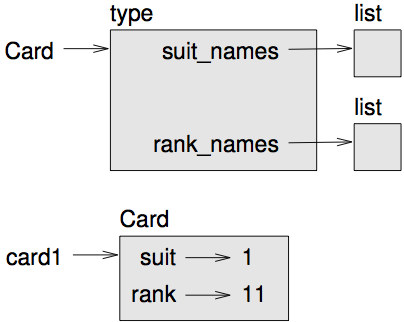
\includegraphics[scale=0.8]{figs/card1.pdf}}
\caption{Object diagram.}
\label{fig.card1}
\end{figure}

Figure~\ref{fig.card1} is a diagram of the {\tt Card} class object
and one Card instance.
\index{state diagram}
\index{diagram!state}
\index{object diagram}
\index{diagram!object}
{\tt Card} is a class object, so it has type {\tt type}.  {\tt
card1} has type {\tt Card}.  (To save space, I didn't draw the
contents of \verb"suit_names" and \verb"rank_names").


\section{Comparing cards}
\label{comparecard}
\index{operator!relational}
\index{relational operator}

For built-in types, there are relational operators
({\tt <}, {\tt >}, {\tt ==}, etc.)
that compare
values and determine when one is greater than, less than, or equal to
another.  For user-defined types, we can override the behavior of
the built-in operators by providing a method named
\verb"__cmp__".  

\verb"__cmp__" takes two parameters, {\tt self} and {\tt other},
and returns a positive number if the first object is greater, a
negative number if the second object is greater, and 0 if they are
equal to each other.
\index{override}
\index{operator overloading}

The correct ordering for cards is not obvious.
For example, which
is better, the 3 of Clubs or the 2 of Diamonds?  One has a higher
rank, but the other has a higher suit.  In order to compare
cards, you have to decide whether rank or suit is more important.

The answer might depend on what game you are playing, but to keep
things simple, we'll make the arbitrary choice that suit is more
important, so all of the Spades outrank all of the Diamonds,
and so on.
\index{cmp method@\_\_cmp\_\_ method}
\index{method!\_\_cmp\_\_}

With that decided, we can write \verb"__cmp__":

\begin{verbatim}
# inside class Card:

    def __cmp__(self, other):
        # check the suits
        if self.suit > other.suit: return 1
        if self.suit < other.suit: return -1

        # suits are the same... check ranks
        if self.rank > other.rank: return 1
        if self.rank < other.rank: return -1

        # ranks are the same... it's a tie
        return 0    
\end{verbatim}
%
You can write this more concisely using tuple comparison:
\index{tuple!comparison}
\index{comparison!tuple}

\begin{verbatim}
# inside class Card:

    def __cmp__(self, other):
        t1 = self.suit, self.rank
        t2 = other.suit, other.rank
        return cmp(t1, t2)
\end{verbatim}
%
The built-in function {\tt cmp} has the same interface as
the method \verb"__cmp__": it takes two values and returns
a positive number if the first is larger, a negative number
if the second is larger, and 0 if they are equal.
\index{cmp function}
\index{function!cmp}

In Python 3, {\tt cmp} no longer exists, and the \verb"__cmp__"
method is not supported.  Instead you should provide \verb"__lt__",
which returns {\tt True} if {\tt self} is less than {\tt other}.
You can implement \verb"__lt__" using tuples and the \verb"<"
operator.

\begin{exercise}

Write a \verb"__cmp__" method for Time objects.  Hint: you
can use tuple comparison, but you also might consider using
integer subtraction.

%    def __cmp__(self, other):
%        return time_to_int(self) - time_to_int(other)

%If {\tt self} is later than {\tt other}, the result is
%a positive number.  If {\tt other} is later, the result
%is negative.  And if {\tt self} and {\tt other} are equal
%(but not necessarily identical)
%the result is zero.

\end{exercise}


\section{Decks}
\index{list!of objects}
\index{deck, playing cards}

Now that we have Cards, the next step is to define Decks.  Since a
deck is made up of cards, it is natural for each Deck to contain a
list of cards as an attribute.
\index{init method}
\index{method!init}

The following is a class definition for {\tt Deck}.  The
init method creates the attribute {\tt cards} and generates
the standard set of fifty-two cards:
\index{composition}
\index{loop!nested}
\index{Deck class}
\index{class!Deck}

\begin{verbatim}
class Deck(object):

    def __init__(self):
        self.cards = []
        for suit in range(4):
            for rank in range(1, 14):
                card = Card(suit, rank)
                self.cards.append(card)
\end{verbatim}
%
The easiest way to populate the deck is with a nested loop.  The outer
loop enumerates the suits from 0 to 3.  The inner loop enumerates the
ranks from 1 to 13.  Each iteration
creates a new Card with the current suit and rank,
and appends it to {\tt self.cards}.
\index{append method}
\index{method!append}


\section{Printing the deck}
\label{printdeck}
\index{str method@\_\_str\_\_ method}
\index{method!\_\_str\_\_}

Here is a \verb"__str__" method for {\tt Deck}:

\begin{verbatim}
#inside class Deck:

    def __str__(self):
        res = []
        for card in self.cards:
            res.append(str(card))
        return '\n'.join(res)
\end{verbatim}
%
This method demonstrates an efficient way to accumulate a large
string: building a list of strings and then using {\tt join}.
The built-in function {\tt str} invokes the \verb"__str__"
method on each card and returns the string representation.
\index{accumulator!string}
\index{string!accumulator}
\index{join method}
\index{method!join}
\index{newline}

Since we invoke {\tt join} on a newline character, the cards
are separated by newlines.  Here's what the result looks like:

\begin{verbatim}
>>> deck = Deck()
>>> print deck
Ace of Clubs
2 of Clubs
3 of Clubs
...
10 of Spades
Jack of Spades
Queen of Spades
King of Spades
\end{verbatim}
%
Even though the result appears on 52 lines, it is
one long string that contains newlines.


\section{Add, remove, shuffle and sort}

To deal cards, we would like a method that
removes a card from the deck and returns it.
The list method {\tt pop} provides a convenient way to do that:
\index{pop method}
\index{method!pop}

\begin{verbatim}
#inside class Deck:

    def pop_card(self):
        return self.cards.pop()
\end{verbatim}
%
Since {\tt pop} removes the {\em last} card in the list, we are
dealing from the bottom of the deck.  In real life ``bottom dealing'' is
frowned upon,
but in this context it's ok.
\index{append method}
\index{method!append}

To add a card, we can use the list method {\tt append}:

\begin{verbatim}
#inside class Deck:

    def add_card(self, card):
        self.cards.append(card)
\end{verbatim}
%
A method like this that uses another function without doing
much real work is sometimes called a {\bf veneer}.  The metaphor
comes from woodworking, where it is common to glue a thin
layer of good quality wood to the surface of a cheaper piece of
wood.
\index{veneer}

In this case we are defining a ``thin'' method that expresses
a list operation in terms that are appropriate for decks.

As another example, we can write a Deck method named {\tt shuffle}
using the function {\tt shuffle} from the {\tt random} module:
\index{random module}
\index{module!random}
\index{shuffle function}
\index{function!shuffle}

\begin{verbatim}
# inside class Deck:
            
    def shuffle(self):
        random.shuffle(self.cards)
\end{verbatim}
%
Don't forget to import {\tt random}.

\begin{exercise}
\index{sort method}
\index{method!sort}

Write a Deck method named {\tt sort} that uses the list method
{\tt sort} to sort the cards in a {\tt Deck}.  {\tt sort} uses
the \verb"__cmp__" method we defined to determine sort order.
\end{exercise}



\section{Inheritance}
\index{inheritance}
\index{object-oriented programming}

The language feature most often associated with object-oriented
programming is {\bf inheritance}.  Inheritance is the ability to
define a new class that is a modified version of an existing
class.
\index{parent class}
\index{child class}
\index{class!child}
\index{subclass}
\index{superclass}

It is called ``inheritance'' because the new class inherits the
methods of the existing class.  Extending this metaphor, the existing
class is called the {\bf parent} and the new class is
called the {\bf child}.

As an example, let's say we want a class to represent a ``hand,''
that is, the set of cards held by one player.  A hand is similar to a
deck: both are made up of a set of cards, and both require operations
like adding and removing cards.

A hand is also different from a deck; there are operations we want for
hands that don't make sense for a deck.  For example, in poker we
might compare two hands to see which one wins.  In bridge, we might
compute a score for a hand in order to make a bid.

This relationship between classes---similar, but different---lends
itself to inheritance.  

The definition of a child class is like other class definitions,
but the name of the parent class appears in parentheses:
\index{parentheses!parent class in}
\index{parent class}
\index{class!parent}
\index{Hand class}
\index{class!Hand}

\begin{verbatim}
class Hand(Deck):
    """Represents a hand of playing cards."""
\end{verbatim}
%
This definition indicates that {\tt Hand} inherits from {\tt Deck};
that means we can use methods like \verb"pop_card" and \verb"add_card"
for Hands as well as Decks.

{\tt Hand} also inherits \verb"__init__" from {\tt Deck}, but
it doesn't really do what we want: instead of populating the hand
with 52 new cards, the init method for Hands should initialize
{\tt cards} with an empty list.
\index{override}
\index{init method}
\index{method!init}

If we provide an init method in the {\tt Hand} class, it overrides the
one in the {\tt Deck} class:

\begin{verbatim}
# inside class Hand:

    def __init__(self, label=''):
        self.cards = []
        self.label = label
\end{verbatim}
%
So when you create a Hand, Python invokes this init method:

\begin{verbatim}
>>> hand = Hand('new hand')
>>> print hand.cards
[]
>>> print hand.label
new hand
\end{verbatim}
%
But the other methods are inherited from {\tt Deck}, so we can use
\verb"pop_card" and \verb"add_card" to deal a card:

\begin{verbatim}
>>> deck = Deck()
>>> card = deck.pop_card()
>>> hand.add_card(card)
>>> print hand
King of Spades
\end{verbatim}
%
A natural next step is to encapsulate this code in a method
called \verb"move_cards":
\index{encapsulation}

\begin{verbatim}
#inside class Deck:

    def move_cards(self, hand, num):
        for i in range(num):
            hand.add_card(self.pop_card())
\end{verbatim}
%
\verb"move_cards" takes two arguments, a Hand object and the number of
cards to deal.  It modifies both {\tt self} and {\tt hand}, and
returns {\tt None}.

In some games, cards are moved from one hand to another,
or from a hand back to the deck.  You can use \verb"move_cards"
for any of these operations: {\tt self} can be either a Deck
or a Hand, and {\tt hand}, despite the name, can also be a {\tt Deck}.

\begin{exercise}

Write a Deck method called \verb"deal_hands" that takes two
parameters, the number of hands and the number of cards per
hand, and that creates new Hand objects, deals the appropriate
number of cards per hand, and returns a list of Hand objects.

\end{exercise}

Inheritance is a useful feature.  Some programs that would be
repetitive without inheritance can be written more elegantly
with it.  Inheritance can facilitate code reuse, since you can
customize the behavior of parent classes without having to modify
them.  In some cases, the inheritance structure reflects the natural
structure of the problem, which makes the program easier to
understand.

On the other hand, inheritance can make programs difficult to read.
When a method is invoked, it is sometimes not clear where to find its
definition.  The relevant code may be scattered among several modules.
Also, many of the things that can be done using inheritance can be
done as well or better without it.  


\section{Class diagrams}
\label{class.diagram}

So far we have seen stack diagrams, which show the state of
a program, and object diagrams, which show the attributes
of an object and their values.  These diagrams represent a snapshot
in the execution of a program, so they change as the program
runs.

They are also highly detailed; for some purposes, too
detailed.  A class diagram is a more abstract representation
of the structure of a program.  Instead of showing individual
objects, it shows classes and the relationships between them.

There are several kinds of relationship between classes:

\begin{itemize}

\item Objects in one class might contain references to objects
in another class.  For example, each Rectangle contains a reference
to a Point, and each Deck contains references to many Cards.
This kind of relationship is called {\bf HAS-A}, as in, ``a Rectangle
has a Point.''

\item One class might inherit from another.  This relationship
is called {\bf IS-A}, as in, ``a Hand is a kind of a Deck.''

\item One class might depend on another in the sense that changes
in one class would require changes in the other.

\end{itemize}
\index{IS-A relationship}
\index{HAS-A relationship}
\index{class diagram}
\index{diagram!class}

A {\bf class diagram} is a graphical representation of these
relationships.  For example, Figure~\ref{fig.class1} shows the
relationships between {\tt Card}, {\tt Deck} and {\tt Hand}.

\begin{figure}
\centerline
{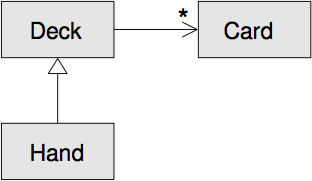
\includegraphics[scale=0.8]{figs/class1.pdf}}
\caption{Class diagram.}
\label{fig.class1}
\end{figure}


The arrow with a hollow triangle head represents an IS-A
relationship; in this case it indicates that Hand inherits
from Deck.

The standard arrow head represents a HAS-A
relationship; in this case a Deck has references to Card
objects.
\index{multiplicity (in class diagram)}

The star ({\tt *}) near the arrow head is a 
{\bf multiplicity}; it indicates how many Cards a Deck has.
A multiplicity can be a simple number, like {\tt 52}, a range,
like {\tt 5..7} or a star, which indicates that a Deck can
have any number of Cards.

A more detailed diagram might show that a Deck actually
contains a {\em list} of Cards, but built-in types
like list and dict are usually not included in class diagrams.

\begin{exercise}

Read {\tt TurtleWorld.py}, {\tt World.py} and {\tt Gui.py}
and draw a class diagram that shows the relationships among
the classes defined there.

\end{exercise}


\section{Debugging}
\index{debugging}

Inheritance can make debugging a challenge because when you
invoke a method on an object, you might not know which method
will be invoked.
\index{polymorphism}

Suppose you are writing a function that works with Hand objects.
You would like it to work with all kinds of Hands, like
PokerHands, BridgeHands, etc.  If you invoke a method like
{\tt shuffle}, you might get the one defined in {\tt Deck},
but if any of the subclasses override this method, you'll
get that version instead.  
\index{flow of execution}

Any time you are unsure about the flow of execution through your
program, the simplest solution is to add print statements at the
beginning of the relevant methods.  If {\tt Deck.shuffle} prints a
message that says something like {\tt Running Deck.shuffle}, then as
the program runs it traces the flow of execution.

As an alternative, you could use this function, which takes an
object and a method name (as a string) and returns the class that
provides the definition of the method:

\begin{verbatim}
def find_defining_class(obj, meth_name):
    for ty in type(obj).mro():
        if meth_name in ty.__dict__:
            return ty
\end{verbatim}
%
Here's an example:

\begin{verbatim}
>>> hand = Hand()
>>> print find_defining_class(hand, 'shuffle')
<class 'Card.Deck'>
\end{verbatim}
%
So the {\tt shuffle} method for this Hand is the one in {\tt Deck}.
\index{mro method}
\index{method!mro}
\index{method resolution order}

\verb"find_defining_class" uses the {\tt mro} method to get the list
of class objects (types) that will be searched for methods.  ``MRO''
stands for ``method resolution order.''
\index{override}
\index{interface}
\index{precondition}
\index{postcondition}

Here's a program design suggestion: whenever you override a method,
the interface of the new method should be the same as the old.  It
should take the same parameters, return the same type, and obey the
same preconditions and postconditions.  If you obey this rule, you
will find that any function designed to work with an instance of a
superclass, like a Deck, will also work with instances of subclasses
like a Hand or PokerHand.

If you violate this rule, your code will collapse like (sorry)
a house of cards.


\section{Data encapsulation}

Chapter~\ref{time} demonstrates a development plan we might call
``object-oriented design.''  We identified objects we needed---{\tt
  Time}, {\tt Point} and {\tt Rectangle}---and defined classes to
represent them.  In each case there is an obvious correspondence
between the object and some entity in the real world (or at least a
mathematical world).
\index{development plan}

But sometimes it is less obvious what objects you need
and how they should interact.  In that case you need a different
development plan.  In the same way that we discovered function
interfaces by encapsulation and generalization, we can discover
class interfaces by {\bf data encapsulation}.
\index{data encapsulation}
\index{encapsulation!data}

Markov analysis, from Section~\ref{markov}, provides a good example.
If you download my code from \url{http://thinkpython.com/code/markov.py},
you'll see that it uses two global variables---\verb"suffix_map" and
\verb"prefix"---that are read and written from several functions.

\begin{verbatim}
suffix_map = {}        
prefix = ()            
\end{verbatim}

Because these variables are global
we can only run one analysis
at a time.  If we read two texts, their prefixes and suffixes would
be added to the same data structures (which makes for some interesting
generated text).

To run multiple analyses, and keep them separate, we can encapsulate
the state of each analysis in an object.
Here's what that looks like:

\begin{verbatim}
class Markov(object):

    def __init__(self):
        self.suffix_map = {}
        self.prefix = ()    
\end{verbatim}

Next, we transform the functions into methods.  For example,
here's \verb"process_word":

\begin{verbatim}
    def process_word(self, word, order=2):
        if len(self.prefix) < order:
            self.prefix += (word,)
            return

        try:
            self.suffix_map[self.prefix].append(word)
        except KeyError:
            # if there is no entry for this prefix, make one
            self.suffix_map[self.prefix] = [word]

        self.prefix = shift(self.prefix, word)        
\end{verbatim}

Transforming a program like this---changing the design without
changing the function---is another example of refactoring
(see Section~\ref{refactoring}).
\index{refactoring}

This example suggests a development plan for designing objects and
methods:

\begin{enumerate}

\item Start by writing functions that read and write global
variables (when necessary).

\item Once you get the program working, look for associations
between global variables and the functions that use them.

\item Encapsulate related variables as attributes of an object.

\item Transform the associated functions into methods of the new
class.

\end{enumerate}


\begin{exercise}

Download my code from Section~\ref{markov}
(\url{http://thinkpython.com/code/markov.py}), and follow the steps described
above to encapsulate the global variables as attributes of a new class
called {\tt Markov}.  Solution: \url{http://thinkpython.com/code/Markov.py}
(note the capital M).

\end{exercise}




\section{Glossary}

\begin{description}

\item[encode:]  To represent one set of values using another
set of values by constructing a mapping between them.
\index{encode}

\item[class attribute:] An attribute associated with a class
object.  Class attributes are defined inside
a class definition but outside any method.
\index{class attribute}
\index{attribute!class}

\item[instance attribute:] An attribute associated with an
instance of a class.
\index{instance attribute}
\index{attribute!instance}

\item[veneer:] A method or function that provides a different
interface to another function without doing much computation.
\index{veneer}

\item[inheritance:] The ability to define a new class that is a
modified version of a previously defined class.
\index{inheritance}

\item[parent class:] The class from which a child class inherits.
\index{parent class}

\item[child class:] A new class created by inheriting from an
existing class; also called a ``subclass.''
\index{child class}
\index{class!child}

\item[IS-A relationship:] The relationship between a child class
and its parent class.
\index{IS-A relationship}

\item[HAS-A relationship:] The relationship between two classes
where instances of one class contain references to instances of
the other.
\index{HAS-A relationship}

\item[class diagram:] A diagram that shows the classes in a program
and the relationships between them.
\index{class diagram}
\index{diagram!class}

\item[multiplicity:] A notation in a class diagram that shows, for
a HAS-A relationship, how many references there are to instances
of another class.
\index{multiplicity (in class diagram)}

\end{description}


\section{Exercises}

\begin{exercise}
\label{poker}

The following are the possible hands in poker, in increasing order
of value (and decreasing order of probability):
\index{poker}

\begin{description}

\item[pair:] two cards with the same rank
\vspace{-0.05in}

\item[two pair:] two pairs of cards with the same rank
\vspace{-0.05in}

\item[three of a kind:] three cards with the same rank
\vspace{-0.05in}

\item[straight:] five cards with ranks in sequence (aces can
be high or low, so {\tt Ace-2-3-4-5} is a straight and so is {\tt
10-Jack-Queen-King-Ace}, but {\tt Queen-King-Ace-2-3} is not.)
\vspace{-0.05in}

\item[flush:] five cards with the same suit
\vspace{-0.05in}

\item[full house:] three cards with one rank, two cards with another
\vspace{-0.05in}

\item[four of a kind:] four cards with the same rank
\vspace{-0.05in}

\item[straight flush:] five cards in sequence (as defined above) and
with the same suit
\vspace{-0.05in}

\end{description}
%
The goal of these exercises is to estimate
the probability of drawing these various hands.

\begin{enumerate}

\item Download the following files from \url{http://thinkpython.com/code}:

\begin{description}

\item[{\tt Card.py}]: A complete version of the {\tt Card},
{\tt Deck} and {\tt Hand} classes in this chapter.

\item[{\tt PokerHand.py}]: An incomplete implementation of a class
that represents a poker hand, and some code that tests it.

\end{description}
%
\item If you run {\tt PokerHand.py}, it deals seven 7-card poker hands
and checks to see if any of them contains a flush.  Read this
code carefully before you go on.

\item Add methods to {\tt PokerHand.py} named \verb"has_pair",
\verb"has_twopair", etc. that return True or False according to
whether or not the hand meets the relevant criteria.  Your code should
work correctly for ``hands'' that contain any number of cards
(although 5 and 7 are the most common sizes).

\item Write a method named {\tt classify} that figures out
the highest-value classification for a hand and sets the
{\tt label} attribute accordingly.  For example, a 7-card hand
might contain a flush and a pair; it should be labeled ``flush''.

\item When you are convinced that your classification methods are
working, the next step is to estimate the probabilities of the various
hands.  Write a function in {\tt PokerHand.py} that shuffles a deck of
cards, divides it into hands, classifies the hands, and counts the
number of times various classifications appear.

\item Print a table of the classifications and their probabilities.
Run your program with larger and larger numbers of hands until the
output values converge to a reasonable degree of accuracy.  Compare
your results to the values at \url{http://en.wikipedia.org/wiki/Hand_rankings}.

\end{enumerate}

Solution: \url{http://thinkpython.com/code/PokerHandSoln.py}.
\end{exercise}


\begin{exercise}
\index{Swampy}
\index{TurtleWorld}

This exercise uses TurtleWorld from Chapter~\ref{turtlechap}.
You will write code that makes Turtles play tag.  If you
are not familiar with the rules of tag, see
\url{http://en.wikipedia.org/wiki/Tag_(game)}.

\begin{enumerate}

\item Download \url{http://thinkpython.com/code/Wobbler.py} and run it.  You
should see a TurtleWorld with three Turtles.  If you press the
{\sf Run} button, the Turtles wander at random.

\item Read the code and make sure you understand how it works.
The {\tt Wobbler} class inherits from {\tt Turtle}, which means
that the {\tt Turtle} methods {\tt lt}, {\tt rt}, {\tt fd}
and {\tt bk} work on Wobblers.

The {\tt step} method gets invoked by TurtleWorld.  It invokes 
{\tt steer}, which turns the Turtle in the desired direction,
{\tt wobble}, which makes a random turn in proportion to the Turtle's
clumsiness, and {\tt move}, which moves forward a few pixels,
depending on the Turtle's speed.
\index{Tagger}

\item Create a file named {\tt Tagger.py}.  Import everything from
  {\tt Wobbler}, then define a class named {\tt Tagger} that inherits
  from {\tt Wobbler}.  Call \verb"make_world" passing the {\tt
    Tagger} class object as an argument.

\item Add a {\tt steer} method to {\tt Tagger} to override the one in
  {\tt Wobbler}.  As a starting place, write a version that always
  points the Turtle toward the origin.  Hint: use the math function
  {\tt atan2} and the Turtle attributes {\tt x}, {\tt y} and
  {\tt heading}.

\item Modify {\tt steer} so that the Turtles stay in bounds.
  For debugging, you might want to use the {\sf Step} button,
  which invokes {\tt step} once on each Turtle.

\item Modify {\tt steer} so that each Turtle points toward its nearest
  neighbor.  Hint: Turtles have an attribute, {\tt world}, that is a
  reference to the TurtleWorld they live in, and the TurtleWorld has
  an attribute, {\tt animals}, that is a list of all Turtles in the
  world.

\item Modify {\tt steer} so the Turtles play tag.  You can add methods
  to {\tt Tagger} and you can override {\tt steer} and
  \verb"__init__", but you may not modify or override {\tt step}, {\tt
    wobble} or {\tt move}.  Also, {\tt steer} is allowed to change the
  heading of the Turtle but not the position.

Adjust the rules and your {\tt steer} method for good quality play;
for example, it should be possible for the slow Turtle to tag the
faster Turtles eventually.

\end{enumerate}

Solution: \url{http://thinkpython.com/code/Tagger.py}.
\end{exercise}



\label{tkinter}

\section{GUI}

Most of the programs we have seen so far are text-based, but
many programs use {\bf graphical user interfaces}, also
known as {\bf GUIs}.
\index{GUI}
\index{graphical user interface}
\index{Tkinter}

Python provides several choices for writing GUI-based programs,
including wxPython, Tkinter, and Qt.  Each has pros and cons, which
is why Python has not converged on a standard.

The one I will present in this chapter is Tkinter because I think
it is the easiest to get started with.  Most of the concepts
in this chapter apply to the other GUI modules, too.

There are several books and web pages about Tkinter.  One of
the best online resources is {\em An Introduction to Tkinter}
by Fredrik Lundh.
\index{Gui module}
\index{module!Gui}
\index{Swampy}

I have written a module called {\tt Gui.py} that comes with
Swampy.  It provides a simplified interface to the functions
and classes in Tkinter.  The examples in this chapter are
based on this module.

Here is a simple example that creates and displays a Gui:

To create a GUI, you have to import {\tt Gui} from Swampy:
%
\begin{verbatim}
from swampy.Gui import *
\end{verbatim}
%
Or, depending on how you installed Swampy, like this:
%
\begin{verbatim}
from Gui import *
\end{verbatim}
%
Then instantiate a Gui object:
%
\begin{verbatim}
g = Gui()
g.title('Gui')
g.mainloop()
\end{verbatim}
%
When you run this code, a window should appear with an empty gray
square and the title {\sf Gui}.  {\tt mainloop} runs the {\bf event
  loop}, which waits for the user to do something and responds
accordingly.  It is an infinite loop; it runs until the user closes
the window, or presses Control-C, or does something that causes the
program to quit.
\index{event loop}
\index{loop!event}
\index{infinite loop}
\index{loop!infinite}

This Gui doesn't do much because it doesn't have any
{\bf widgets}.  Widgets are the elements that make up a
GUI; they include:
\index{widget}

\begin{description}

\item[Button:] A widget, containing text or an image, that
performs an action when pressed.

\item[Canvas:] A region that can display lines, rectangles,
circles and other shapes.

\item[Entry:] A region where users can type text.

\item[Scrollbar:] A widget that controls the visible part of another
widget.

\item[Frame:] A container, often invisible, that contains other
widgets.

\end{description}

The empty gray square you see when you create a Gui is
a Frame.  When you create a new widget, it is added to this Frame.



\section{Buttons and callbacks}
\index{Button widget}
\index{widget!Button}

The method {\tt bu} creates a Button widget:

\begin{verbatim}
button = g.bu(text='Press me.')
\end{verbatim}
%
The return value from {\tt bu} is a Button object.  The button
that appears in the Frame is a graphical representation of this
object; you can control the button by invoking methods on it.
\index{option}

{\tt bu} takes up to 32 parameters that control the appearance
and function of the button.  These parameters are called
{\bf options}.  Instead of providing values for all 32 options,
you can use keyword arguments, like \verb"text='Press me.'",
to specify only the options you need and use the default
values for the rest.
\index{keyword argument}
\index{argument!keyword}

When you add a widget to the Frame, it gets ``shrink-wrapped;''
that is, the Frame shrinks to the size of the Button.  If you
add more widgets, the Frame grows to accommodate them.
\index{Label widget}
\index{widget!Label}

The method {\tt la} creates a Label widget:

\begin{verbatim}
label = g.la(text='Press the button.')
\end{verbatim}
%
By default, Tkinter stacks the widgets top-to-bottom and centers
them.  We'll see how to override that behavior soon.

If you press the button, you will see that it doesn't do much.
That's because you haven't ``wired it up;'' that is, you haven't
told it what to do!

The option that controls the behavior of a button is {\tt command}.
The value of {\tt command} is a function that gets executed when
the button is pressed.  For example, here is a function that creates
a new Label:

\begin{verbatim}
def make_label():
    g.la(text='Thank you.')
\end{verbatim}
%
Now we can create a button with this function as its command:

\begin{verbatim}
button2 = g.bu(text='No, press me!', command=make_label)
\end{verbatim}
%
When you press this button, it should execute \verb"make_label"
and a new label should appear.
\index{callback}

The value of the {\tt command} option
is a function object, which is known as a {\bf callback} because
after you call {\tt bu} to create the button, the flow of execution
``calls back'' when the user presses the button.
\index{event-driven programming}

This kind of flow is characteristic of {\bf event-driven programming}.
User actions, like button presses and key strokes, are called {\bf
events}.  In event-driven programming, the flow of execution is
determined by user actions rather than by the programmer.  

The challenge of event-driven programming is to construct a set of
widgets and callbacks that work correctly (or at least generate
appropriate error messages) for any sequence of user actions.

\begin{exercise}

Write a program that creates a GUI with a single button.  When the
button is pressed it should create a second button.  When
{\em that} button is pressed, it should create a label that
says, ``Nice job!''.

What happens if you press the buttons more than once?
Solution: \url{http://thinkpython.com/code/button_demo.py}

\end{exercise}


\section{Canvas widgets}
\index{Canvas widget}
\index{widget!Canvas}

One of the most versatile widgets is the Canvas, which creates
a region for drawing lines, circles and other shapes.  If you
did Exercise~\ref{canvas} you are already familiar with canvases.

The method {\tt ca} creates a new Canvas:

\begin{verbatim}
canvas = g.ca(width=500, height=500)
\end{verbatim}
%
{\tt width} and {\tt height} are the dimensions of the canvas
in pixels.  
\index{config method}
\index{method!config}

After you create a widget, you can still change the values of
the options with the
{\tt config} method.  For example, the {\tt bg} option changes
the background color:

\begin{verbatim}
canvas.config(bg='white')
\end{verbatim}
%
The value of {\tt bg} is a string
that names a color.  The set of legal color names is different
for different implementations of Python, but all implementations
provide at least:

\begin{verbatim}
white   black
red     green    blue   
cyan    yellow   magenta
\end{verbatim}
%
Shapes on a Canvas are called {\bf items}.  For example,
the Canvas method {\tt circle} draws (you guessed it) a circle:
\index{Canvas item}
\index{item!Canvas}

\begin{verbatim}
item = canvas.circle([0,0], 100, fill='red')
\end{verbatim}
%
The first argument is a coordinate pair that specifies the
center of the circle; the second is the radius.
\index{Canvas coordinate}
\index{coordinate!Canvas}

{\tt Gui.py} provides a standard Cartesian coordinate system with
the origin at the center of the Canvas and the positive $y$ axis
pointing up.  This is different from some other graphics systems
where the origin is in the upper left corner, with the $y$ axis
pointing down.

The {\tt fill} option specifies that the circle should be filled
in with red.

The return value from {\tt circle} is an Item object that
provides methods for modifying the item on the canvas.  For
example, you can use {\tt config} to change any of the circle's
options:

\begin{verbatim}
item.config(fill='yellow', outline='orange', width=10)
\end{verbatim}
%
{\tt width} is the thickness of the outline in pixels;
{\tt outline} is the color.

\begin{exercise}
\label{circle}

Write a program that creates a Canvas and a Button.  When the
user presses the Button, it should draw a circle on the canvas.

\end{exercise}


\section{Coordinate sequences}
\index{coordinate sequence}
\index{sequence!coordinate}

The {\tt rectangle} method takes a sequence of coordinates that
specify opposite corners of the rectangle.  This example
draws a blue rectangle with the lower left corner at the origin
and the upper right corner at $(200,100)$:

\begin{verbatim}
canvas.rectangle([[0, 0], [200, 100]], 
                 fill='blue', outline='orange', width=10)
\end{verbatim}
%
This way of specifying corners is called
a {\bf bounding box} because the two points
bound the rectangle.
\index{bounding box}

{\tt oval} takes a bounding box and draws an oval
within the specified rectangle:

\begin{verbatim}
canvas.oval([[0, 0], [200, 100]], outline='orange', width=10)
\end{verbatim}
%
{\tt line} takes a sequence of coordinates and draws
a line that connects the points.  This example draws two legs
of a triangle:

\begin{verbatim}
canvas.line([[0, 100], [100, 200], [200, 100]], width=10)
\end{verbatim}
%
{\tt polygon} takes the same arguments, but it draws the last
leg of the polygon (if necessary) and fills it in:

\begin{verbatim}
canvas.polygon([[0, 100], [100, 200], [200, 100]],
               fill='red', outline='orange', width=10)
\end{verbatim}
%


\section{More widgets}
\index{Text widget}
\index{widget!Text}

Tkinter provides two widgets that let users type text: an
Entry, which is a single line, and a Text widget, which has
multiple lines.
\index{Entry widget}
\index{widget!Entry}

{\tt en} creates a new Entry:

\begin{verbatim}
entry = g.en(text='Default text.')
\end{verbatim}
%
The {\tt text} option allows you to put text into the entry
when it is created.  The {\tt get} method returns the contents
of the Entry (which may have been changed by the user):

\begin{verbatim}
>>> entry.get()
'Default text.'
\end{verbatim}
%
{\tt te} creates a Text widget:

\begin{verbatim}
text = g.te(width=100, height=5)
\end{verbatim}
%
{\tt width} and {\tt height} are the dimensions of the
widget in characters and lines.

{\tt insert} puts text into the Text widget:

\begin{verbatim}
text.insert(END, 'A line of text.')
\end{verbatim}
%
{\tt END} is a special index that indicates the last character in the
Text widget.

You can also specify a character using a dotted index, like {\tt 1.1},
which has the line number before the dot and the column number after.
The following example adds the letters \verb"'nother'" after the first
character of the first line.

\begin{verbatim}
>>> text.insert(1.1, 'nother')
\end{verbatim}
%
The {\tt get} method reads the text in the widget; it takes a start
and end index as arguments.  The following example returns all the
text in the widget, including the newline character:

\begin{verbatim}
>>> text.get(0.0, END)
'Another line of text.\n'
\end{verbatim}
%
The {\tt delete} method removes text from the widget;
the following example deletes all but the first two characters:

\begin{verbatim}
>>> text.delete(1.2, END)
>>> text.get(0.0, END)
'An\n'
\end{verbatim}
%

\begin{exercise}
\label{circle2}

Modify your solution to Exercise~\ref{circle} by adding an
Entry widget and a second button.  When the user presses the
second button, it should read a color name from the Entry and
use it to change the fill color of the circle.  Use {\tt config}
to modify the existing circle; don't create a new one.

Your program should handle the case where the user tries to
change the color of a circle that hasn't been created, and
the case where the color name is invalid.

You can see my solution at \url{http://thinkpython.com/code/circle_demo.py}.

\end{exercise}


\section{Packing widgets}

So far we have been stacking widgets in a single column, but in most
GUIs the layout is more complicated.  For example,
Figure~\ref{fig.turtleworld} shows a simplified version of
TurtleWorld (see Chapter~\ref{turtlechap}).

\begin{figure}
\centerline{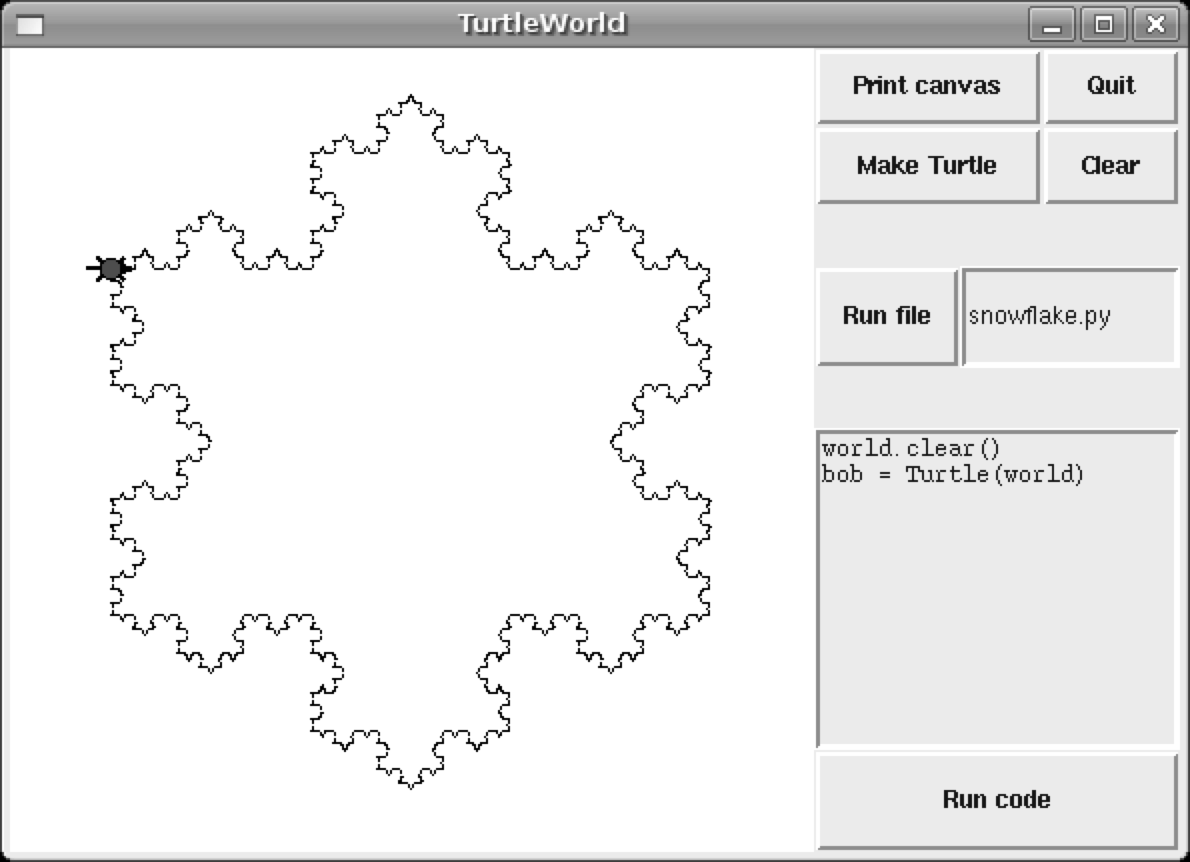
\includegraphics[scale=0.5]{figs/TurtleWorld.pdf}}
\caption{TurtleWorld after running the snowflake code.}
\label{fig.turtleworld}
\end{figure}


This section presents the code that creates this GUI, broken into a
series of steps.  You can download the complete example
from \url{http://thinkpython.com/code/SimpleTurtleWorld.py}.

At the top level, this GUI contains two widgets---a Canvas and a
Frame---arranged in a row.  So the first step is to create the row.
\index{SimpleTurtleWorld class}
\index{class!SimpleTurtleWorld}

\begin{verbatim}
class SimpleTurtleWorld(TurtleWorld):
    """This class is identical to TurtleWorld, but the code that
    lays out the GUI is simplified for explanatory purposes."""

    def setup(self):
        self.row()
        ...
\end{verbatim}
%
{\tt setup} is the function that creates and arranges the widgets.
Arranging widgets in a GUI is called {\bf packing}.
\index{packing widgets}
\index{widget, packing}
\index{Frame widget}
\index{widget!Frame}

{\tt row} creates a row Frame and makes it the ``current Frame.''
Until this Frame is closed or another Frame is created, all
subsequent widgets are packed in a row.

Here is the code that creates the Canvas and the column Frame
that hold the other widgets:

\begin{verbatim}
        self.canvas = self.ca(width=400, height=400, bg='white')
        self.col()
\end{verbatim}
%
The first widget in the column is a grid Frame, which contains
four buttons arranged two-by-two:

\begin{verbatim}
        self.gr(cols=2)
        self.bu(text='Print canvas', command=self.canvas.dump)
        self.bu(text='Quit', command=self.quit)
        self.bu(text='Make Turtle', command=self.make_turtle)
        self.bu(text='Clear', command=self.clear)
        self.endgr()
\end{verbatim}
%
{\tt gr} creates the grid; the argument is the number of
columns.  Widgets in the grid are
laid out left-to-right, top-to-bottom.
\index{callback}
\index{bound method}
\index{method, bound}
\index{subject}

The first button uses {\tt self.canvas.dump} as a callback; the second
uses {\tt self.quit}.  These are {\bf bound methods}, which means they
are associated with a particular object.  When they are invoked, they
are invoked on the object.

The next widget in the column is a row Frame that contains
a Button and an Entry:

\begin{verbatim}
        self.row([0,1], pady=30)
        self.bu(text='Run file', command=self.run_file)
        self.en_file = self.en(text='snowflake.py', width=5)
        self.endrow()
\end{verbatim}
%
The first argument to {\tt row} is a list of weights that
determines how extra space is allocated between widgets.  
The list {\tt [0,1]} means that all extra space is allocated
to the second widget, which is the Entry.  If you run this code
and resize the window, you will see that the Entry grows and
the Button doesn't.

The option {\tt pady} ``pads'' this row in the $y$ direction,
adding 30 pixels of space above and below.

{\tt endrow} ends this row of widgets, so subsequent widgets are
packed in the column Frame.  {\tt Gui.py} keeps a stack of Frames:

\begin{itemize}

\item When you use {\tt row}, {\tt col} or {\tt gr} to create a Frame,
it goes on top of the stack and becomes the current Frame.

\item When you use {\tt endrow}, {\tt endcol} or {\tt endgr} to close
a Frame, it gets popped off the stack and the previous Frame on the
stack becomes the current Frame.

\end{itemize} 

The method \verb"run_file" reads the contents of the Entry,
uses it as a filename, reads the contents
and passes it to \verb"run_code".  {\tt self.inter} is an
Interpreter object that knows how to take a string and
execute it as Python code.

\begin{verbatim}
    def run_file(self):
        filename = self.en_file.get()
        fp = open(filename)
        source = fp.read()
        self.inter.run_code(source, filename)
\end{verbatim}
%
The last two widgets are a Text widget and a Button:

\begin{verbatim}
        self.te_code = self.te(width=25, height=10)
        self.te_code.insert(END, 'world.clear()\n')
        self.te_code.insert(END, 'bob = Turtle(world)\n')

        self.bu(text='Run code', command=self.run_text)
\end{verbatim}
%
\verb"run_text" is similar to \verb"run_file" except that it takes
the code from the Text widget instead of from a file:

\begin{verbatim}
    def run_text(self):
        source = self.te_code.get(1.0, END)
        self.inter.run_code(source, '<user-provided code>')
\end{verbatim}
%
Unfortunately, the details of widget layout are different in
other languages, and in different Python modules.
Tkinter alone provides three different mechanisms for arranging
widgets.  These mechanisms are called {\bf geometry managers}.
The one I demonstrated in this section is the ``grid'' geometry
manager; the others are called ``pack'' and ``place''.
\index{geometry manager}

Fortunately, most of the concepts in this section apply to
other GUI modules and other languages.


\section{Menus and Callables}
\index{Menubutton widget}
\index{widget!Menubutton}

A Menubutton is a widget that looks like a button, but when pressed
it pops up a menu.  After the user selects an item, the menu
disappears.

Here is code that creates a color selection Menubutton
(you can download it from \url{http://thinkpython.com/code/menubutton_demo.py}):

\begin{verbatim}
g = Gui()
g.la('Select a color:')
colors = ['red', 'green', 'blue']
mb = g.mb(text=colors[0])
\end{verbatim}
%
{\tt mb} creates the Menubutton.  Initially, the text on the button is
the name of the default color.  The following loop creates one menu
item for each color:

\begin{verbatim}
for color in colors:
    g.mi(mb, text=color, command=Callable(set_color, color))
\end{verbatim}
%
The first argument of {\tt mi} is the Menubutton these items are
associated with.
\index{callback}
\index{Callable object}
\index{object!Callable}

The {\tt command} option is a Callable object, which is something new.
So far we have seen functions and bound methods used as callbacks,
which works fine if you don't have to pass any arguments to
the function.  Otherwise you have to construct a Callable object
that contains a function, like \verb"set_color", and its arguments,
like {\tt color}.

The Callable object stores a reference to the function and the
arguments as attributes.  Later, when the user clicks on a menu
item, the callback calls the function and passes the stored
arguments.

Here is what \verb"set_color" might look like:

\begin{verbatim}
def set_color(color):
    mb.config(text=color)
    print color
\end{verbatim}
%
When the user selects a menu item and \verb"set_color" is called,
it configures the Menubutton to display the newly-selected color.
It also print the color; if you try this example, you can confirm that
\verb"set_color" is called when you select an item (and {\em not}
called when you create the Callable object).


\section{Binding}
\index{binding}
\index{callback}

A {\bf binding} is an association between a widget, an event and a
callback: when an event (like a button press) happens on a widget, the
callback is invoked.

Many widgets have default bindings.  For example, when you press
a button, the default binding changes the relief of the button
to make it look depressed.  When you release the button, the
binding restores the appearance of the button and invokes the
callback specified with the {\tt command} option.

You can use the {\tt bind} method to override these default
bindings or to add new ones.  For example, this code creates a
binding for a canvas (you can download the code in this
section from \url{http://thinkpython.com/code/draggable_demo.py}):

\begin{verbatim}
ca.bind('<ButtonPress-1>', make_circle)
\end{verbatim}
%
The first argument is an event string; this event is triggered
when the user presses the left mouse button.  Other mouse
events include {\tt ButtonMotion}, {\tt ButtonRelease} and
{\tt Double-Button}.
\index{event string}
\index{event handler}

The second argument is an event handler.  An event handler
is a function or bound method, like a callback, but an important
difference is that an event handler takes an Event object as a
parameter.  Here is an example:

\begin{verbatim}
def make_circle(event):
    pos = ca.canvas_coords([event.x, event.y])
    item = ca.circle(pos, 5, fill='red')
\end{verbatim}
%
The Event object contains information about the type of event and
details like the coordinates of the mouse pointer.  In this example
the information we need is
the location of the mouse click.  These
values are in ``pixel coordinates,'' which are defined by the
underlying graphical system.  The method \verb"canvas_coords"
translates them to ``Canvas coordinates,'' which are compatible with
Canvas methods like {\tt circle}.
\index{Event object}
\index{object!Event}

For Entry widgets, it is common to bind the \verb"<Return>" event,
which is triggered when the user presses the {\sf Return} or
{\sf Enter} key.  For example, the following code creates a Button
and an Entry.

\begin{verbatim}
bu = g.bu('Make text item:', make_text)
en = g.en()
en.bind('<Return>', make_text)
\end{verbatim}
%
\verb"make_text" is called when the Button is pressed or when
the user hits {\sf Return} while typing in the Entry.  To make
this work, we need a function that can be called as a command
(with no arguments) or as an event handler (with an Event
as an argument):

\begin{verbatim}
def make_text(event=None):
    text = en.get()
    item = ca.text([0,0], text)
\end{verbatim}
%
\verb"make_text" gets the contents of the Entry and displays
it as a Text item in the Canvas.

It is also possible to create bindings for Canvas items.
The following is a class definition for {\tt Draggable},
which is a child class of {\tt Item} that provides bindings
that implement drag-and-drop capability.
\index{drag-and-drop}

\begin{verbatim}
class Draggable(Item):

    def __init__(self, item):
        self.canvas = item.canvas
        self.tag = item.tag
        self.bind('<Button-3>', self.select)
        self.bind('<B3-Motion>', self.drag)
        self.bind('<Release-3>', self.drop)
\end{verbatim}
%
The init method takes an Item as a parameter.  It copies
the attributes of the Item and then creates bindings for
three events: a button press, button motion, and button release.

The event handler {\tt select} stores the coordinates
of the current event and the original color of the item, then
changes the color to yellow:

\begin{verbatim}
    def select(self, event):
        self.dragx = event.x
        self.dragy = event.y

        self.fill = self.cget('fill')
        self.config(fill='yellow')
\end{verbatim}
%
{\tt cget} stands for ``get configuration;'' it takes the name of an
option as a string and returns the current value of that option.

{\tt drag} computes how far the object has moved relative to the
starting place, updates the stored coordinates, and then moves the
item.
\index{update!coordinate}

\begin{verbatim}
    def drag(self, event):
        dx = event.x - self.dragx
        dy = event.y - self.dragy

        self.dragx = event.x
        self.dragy = event.y

        self.move(dx, dy)
\end{verbatim}
%
This computation is done in pixel coordinates; there is no need to
convert to Canvas coordinates.
\index{Canvas coordinate}
\index{coordinate!Canvas}
\index{pixel coordinate}
\index{coordinate!pixel}

Finally, {\tt drop} restores the original color of the item:

\begin{verbatim}
    def drop(self, event):
        self.config(fill=self.fill)
\end{verbatim}
%
You can use the {\tt Draggable} class to add drag-and-drop
capability to an existing item.  For example, here is a modified
version of \verb"make_circle" that uses {\tt circle} to create
an Item and {\tt Draggable} to make it draggable:

\begin{verbatim}
def make_circle(event):
    pos = ca.canvas_coords([event.x, event.y])
    item = ca.circle(pos, 5, fill='red')
    item = Draggable(item)
\end{verbatim}
%
This example demonstrates one of the benefits of inheritance: you can
modify the capabilities of a parent class without modifying its
definition.  This is particularly useful if you want to change
behavior defined in a module you did not write.


\section{Debugging}
\index{debugging}

One of the challenges of GUI programming is keeping track of
which things happen while the GUI is being built and which
things happen later in response to user events.
\index{callback}

For example, when you are setting up a callback, it is a common error
to call the function rather than passing a reference to it:

\begin{verbatim}
def the_callback():
    print 'Called.'

g.bu(text='This is wrong!', command=the_callback())
\end{verbatim}
%
If you run this code, you will see that it calls \verb"the_callback"
immediately, and {\em then} creates the button.  When you press the
button, it does nothing because the return value from 
\verb"the_callback" is {\tt None}.
Usually you do not want to invoke a callback while you are
setting up the GUI; it should only be invoked later in response to
a user event.
\index{flow of execution}
\index{event-driven programming}

Another challenge of GUI programming is that you don't have control
of the flow of execution.  Which parts of the program execute
and their order are determined by user actions.
That means that you have to design your program to work correctly
for any possible sequence of events.

For example, the GUI in Exercise~\ref{circle2} has two widgets:
one creates a Circle item and the other changes the color of the
Circle.  If the user creates the circle and then changes its color,
there's no problem.  But what if the user changes the color of
a circle that doesn't exist yet?  Or creates more than one circle?

As the number of widgets grows, it is increasingly difficult to
imagine all possible sequences of events.  One way to manage this 
complexity is to encapsulate the state of the system in an object
and then consider:

\begin{itemize}

\item What are the possible states?  In the Circle example, we
might consider two states: before and after the user creates the
first circle.

\item In each state, what events can occur?  In the example,
the user can press either of the buttons, or quit.

\item For each state-event pair, what is the desired outcome?
Since there are two states and two buttons, there are four
state-event pairs to consider.

\item What can cause a transition from one state to another?
In this case, there is a transition when the user creates
the first circle.

\end{itemize}

You might also find it useful to define, and check, invariants that
should hold regardless of the sequence of events.
\index{invariant}

This approach to GUI programming can help you write correct
code without taking the time to test every possible sequence
of user events!


\section{Glossary}

\begin{description}

\item[GUI:] A graphical user interface.
\index{GUI}

\item[widget:] One of the elements that makes up a GUI, including
buttons, menus, text entry fields, etc. 
\index{widget}

\item[option:] A value that controls the appearance or function of
a widget.
\index{option}

\item[keyword argument:] An argument that indicates the parameter
name as part of the function call.
\index{keyword argument}

\item[callback:] A function associated with a widget that is
called when the user performs an action.
\index{callback}

\item[bound method:] A method associated with a particular instance.
\index{bound method}

\item[event-driven programming:] A style of programming in which
the flow of execution is determined by user actions.
\index{event-driven programming}

\item[event:] A user action, like a mouse click or key press, that
causes a GUI to respond.
\index{event}

\item[event loop:] An infinite loop that waits for user actions
and responds.
\index{event loop}

\item[item:] A graphical element on a Canvas widget.
\index{item!Canvas}

\item[bounding box:] A rectangle that encloses a set of items,
usually specified by two opposing corners.
\index{bounding box}

\item[pack:] To arrange and display the elements of a GUI.
\index{packing widgets}

\item[geometry manager:] A system for packing widgets.
\index{geometry manager}

\item[binding:] An association between a widget, an event, and
an event handler.  The event handler is called when the event
occurs in the widget.
\index{binding}

\end{description}


\section{Exercises}

\begin{exercise}
\index{image viewer}

For this exercise, you will write an image viewer.  Here is
a simple example:

\begin{verbatim}
g = Gui()
canvas = g.ca(width=300)
photo = PhotoImage(file='danger.gif')
canvas.image([0,0], image=photo)
g.mainloop()
\end{verbatim}
%
{\tt PhotoImage} reads a file and returns a {\tt PhotoImage} object
that Tkinter can display.  {\tt Canvas.image} puts the image on the
canvas, centered on the given coordinates.  You can also put images on
labels, buttons, and some other widgets:

\begin{verbatim}
g.la(image=photo)
g.bu(image=photo)
\end{verbatim}
%
PhotoImage can only handle a few image formats, like GIF and PPM, 
but we can use the Python Imaging Library (PIL) to read other
files.
\index{Python Imaging Library (PIL)}
\index{PIL (Python Imaging Library)}
\index{Image module}
\index{module!Image}

The name of the PIL module is {\tt Image}, but Tkinter defines an
object with the same name.  To avoid the conflict, you can use {\tt
  import...as} like this:

\begin{verbatim}
import Image as PIL
import ImageTk
\end{verbatim}
%
The first line imports {\tt Image} and
gives it the local name {\tt PIL}.  The second
line imports {\tt ImageTk}, which can translate a PIL
image into a Tkinter PhotoImage.  Here's an example:

\begin{verbatim}
image = PIL.open('allen.png')
photo2 = ImageTk.PhotoImage(image)
g.la(image=photo2)
\end{verbatim}
%

\begin{enumerate}

\item Download \verb"image_demo.py", \verb"danger.gif" and \verb"allen.png"
from \url{http://thinkpython.com/code}.  Run \verb"image_demo.py".  You
might have to install {\tt PIL} and {\tt ImageTk}.  
They are probably in your software repository,  but if not
you can get them from \url{http://pythonware.com/products/pil}.

\item In \verb"image_demo.py" change the name of the second
PhotoImage from {\tt photo2} to {\tt photo} and run the program
again.  You should see the second PhotoImage but not the first.

The problem is that when you reassign {\tt photo} it overwrites
the reference to the first PhotoImage, which then disappears.  The
same thing happens if you assign a PhotoImage to a local
variable; it disappears when the function ends.

To avoid this problem, you have to store a reference to each
PhotoImage you want to keep.  You can use a global variable, or
store PhotoImages in a data structure or as an attribute of
an object.

This behavior can be frustrating, which is why I am warning
you (and why the example image says ``Danger!'').
\index{bug!worst ever}
\index{worst bug!ever}

\item Starting with this example, write a program that takes
the name of a directory and loops through all the files, displaying
any files that PIL recognizes as images.  You can use a {\tt try}
statement to catch the files PIL doesn't recognize.

When the user clicks on the image, the program should display the next one.

\item PIL provides a variety of methods for manipulating images.
You can read about them at \url{http://pythonware.com/library/pil/handbook}.
As a challenge, choose a few of these methods and provide a
GUI for applying them to images.

\end{enumerate}

Solution: \url{http://thinkpython.com/code/ImageBrowser.py}.

\end{exercise}


\begin{exercise}
\index{vector graphics}
\index{SVG}

A vector graphics editor is a program that allows users to draw and
edit shapes on the screen and generate output files in vector graphics
formats like Postscript and SVG.

Write a simple vector graphics editor using Tkinter.  At a
minimum, it should allow users to draw lines, circles and
rectangles, and it should use {\tt Canvas.dump} to
generate a Postscript description of the contents of the
Canvas.

As a challenge, you could allow users to select and resize
items on the Canvas.

% TODO: write a solution!

\end{exercise}


\begin{exercise}

Use Tkinter to write a basic web browser.  It
should have a Text widget where the user can enter a URL
and a Canvas to display the contents of the page.
\index{urllib module}
\index{module!urllib}
\index{URL}
\index{HTMLParser module}
\index{module!HTMLParser}

You can use the {\tt urllib} module to download files
(see Exercise~\ref{urllib}) and
the {\tt HTMLParser} module to parse the HTML
tags (see \url{http://docs.python.org/2/library/htmlparser.html}).
\index{plain text}
\index{text!plain}
\index{hyperlink}

At a minimum your browser should handle plain text and hyperlinks.  As
a challenge you could handle background colors, text
formatting tags and images.

% TODO: write a solution!

\end{exercise}



\appendix

